\documentclass[12pt]{article}
%--------------------   start of the 'preamble'
%
\usepackage{graphicx,amssymb,amstext,amsmath,color}
\usepackage{grffile}
\usepackage[margin=2cm]{geometry}
\usepackage{abstract}
\usepackage{setspace}
\usepackage[footnotesize,bf]{caption}

% TABLE
\usepackage{multicol,hhline,colortbl,multirow}
\usepackage{braket}
\usepackage{siunitx}
\usepackage{hyperref}
\usepackage{authblk}
\usepackage{siunitx}
\usepackage{adjustbox}
\usepackage{mathrsfs}
%%\usepackage[sort&compress]{natbib}
%%\bibpunct{(}{)}{,}{a}{, }{;}
%
\usepackage[sort&compress]{natbib}
\bibpunct{[}{]}{,}{s}{}{;}


\definecolor{gray}{gray}{0.8}
\def\mobunits{\square\centi\meter\per\volt\per\second}
\def\gcm{\gram\per\cubic\centi\meter}
\def\ccg{\cellcolor{gray}}

\renewcommand{\labelitemii}{$\circ$}
\renewcommand{\bibname}{References}


\title{What Effect Does Fully Equilibrating After Fine-Graining Have on the Charge Transport Properties?}
\author{Matthew Jones}
\date{\today}

\begin{document}
\maketitle


\section{Mobilities}

\begin{center}
\begin{adjustbox}{max width = \textwidth}
\begin{tabular}{| c | c | c | c | c | c | c |}
\hline
\rule{0pt}{2.5ex} 
\multirow{2}{*}{\textbf{ID}}&\multirow{2}{*}{\textbf{Simulation Name}}&\textbf{Density}&\textbf{Anisotropy}&\textbf{Stacks}&\textbf{Stack Threshold}&\textbf{Mobility}\\
                            &&(\SI{}{\gcm})&(Arb. U.)&(Arb. U.)&(\AA)&(\SI{}{\mobunits})\\
\hhline{|=======|}
\textbf{1}&\rule{0pt}{2.5ex}equilP3HT\_1.5&1.676&0.2201&1&7.0845&$1.18\times 10^{1}$\\
\textbf{\ccg2}&\rule{0pt}{2.5ex}{\ccg}equilP3HT\_1.75&\ccg1.061&\ccg0.0105&\ccg1&\ccg4.67&\ccg8.05$\times 10^{-1}$\\
\textbf{3}&\rule{0pt}{2.5ex}equilP3HT\_2.0&0.892&0.0068&4&4.8388&$5.17\times 10^{-1}$\\
\textbf{\ccg4}&\rule{0pt}{2.5ex}{\ccg}equilP3HT\_2.25&\ccg0.787&\ccg0.0050&\ccg42&\ccg4.6085&\ccg3.77$\times 10^{-1}$\\
\textbf{5}&\rule{0pt}{2.5ex}equilP3HT\_2.5&0.685&0.0097&64&4.8188&$2.43\times 10^{-1}$\\
\hhline{|=======|}
\textbf{\ccg6}&\rule{0pt}{2.5ex}{\ccg}origP3HT\_T1.5&\ccg1.676&\ccg0.1282&\ccg1&\ccg7.3947&\ccg1.17$\times 10^{1}$\\
\textbf{7}&\rule{0pt}{2.5ex}origP3HT\_1.75&1.061&0.0197&19&4.4702&$3.48\times 10^{-1}$\\
\textbf{\ccg8}&\rule{0pt}{2.5ex}{\ccg}origP3HT\_2.0&\ccg0.892&\ccg0.0085&\ccg1&\ccg5.0683&\ccg4.46$\times 10^{-1}$\\
\textbf{9}&\rule{0pt}{2.5ex}origP3HT\_2.25&0.787&0.0114&5&4.7747&$5.52\times 10^{-1}$\\
\textbf{\ccg10}&\rule{0pt}{2.5ex}{\ccg}origP3HT\_2.5&\ccg0.685&\ccg0.0188&\ccg25&\ccg4.8465&\ccg4.03$\times 10^{-1}$\\
\hhline{-------}
\end{tabular}\label{table:mob}
\end{adjustbox}
\captionof{table}{The results from MorphCT for the usual P3HT morphologies, with Voronoi neighbours. Runs \textbf{1}-\textbf{5} are the previous Voronoi systems (where the systems were run for 1E5 timesteps during the final fine-graining phase), whereas runs \textbf{6}-\textbf{10} have been equilibrated for 1E7 timesteps during the final fine-graining phase.}
\end{center}


\begin{figure}[h!]\centering
    \begin{tabular}{cc}
        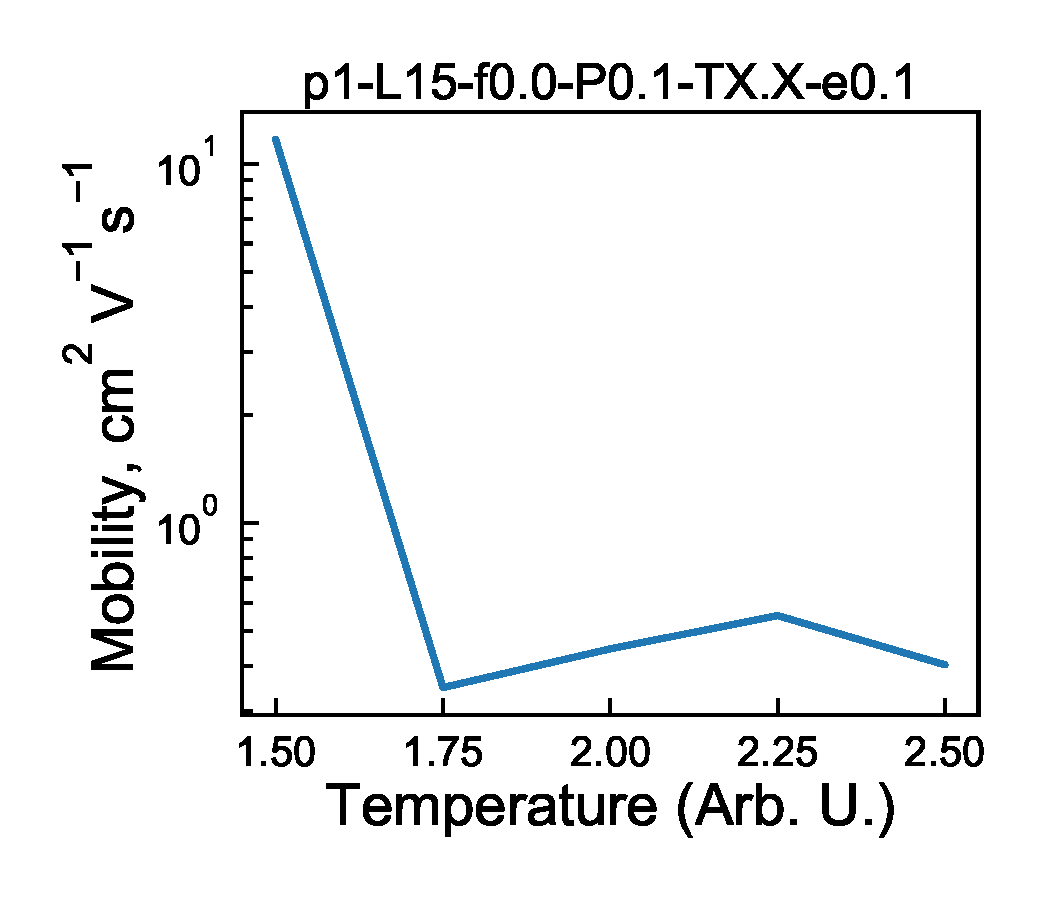
\includegraphics[width=0.5\textwidth]{Figures/origP3HTMob.pdf}&
        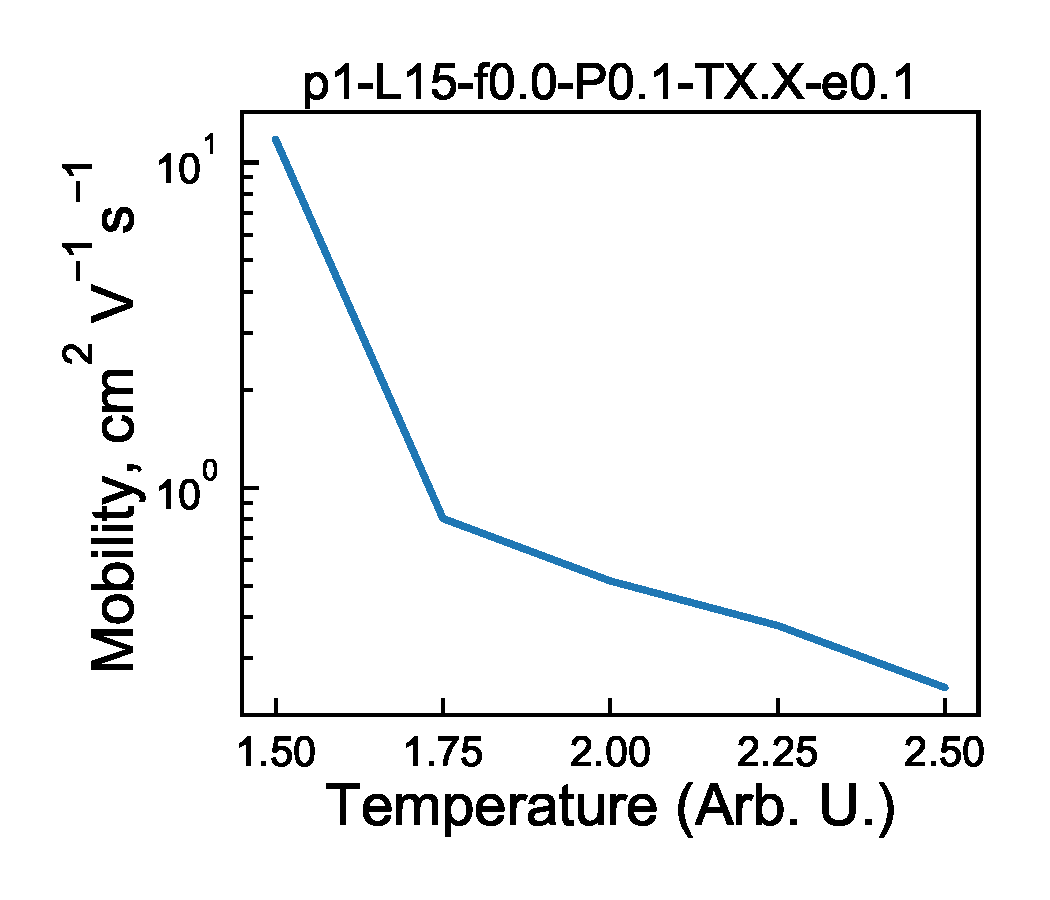
\includegraphics[width=0.5\textwidth]{Figures/equilP3HTMob.pdf}
    \end{tabular}
    \caption{The evolution of the mobility of the p1-L15-f0.0-P0.1-TX.X-e0.5 systems.
}
	\label{fig:mob}
\end{figure}

\clearpage

\section{Equilibration}


\begin{figure}[h!]\centering
	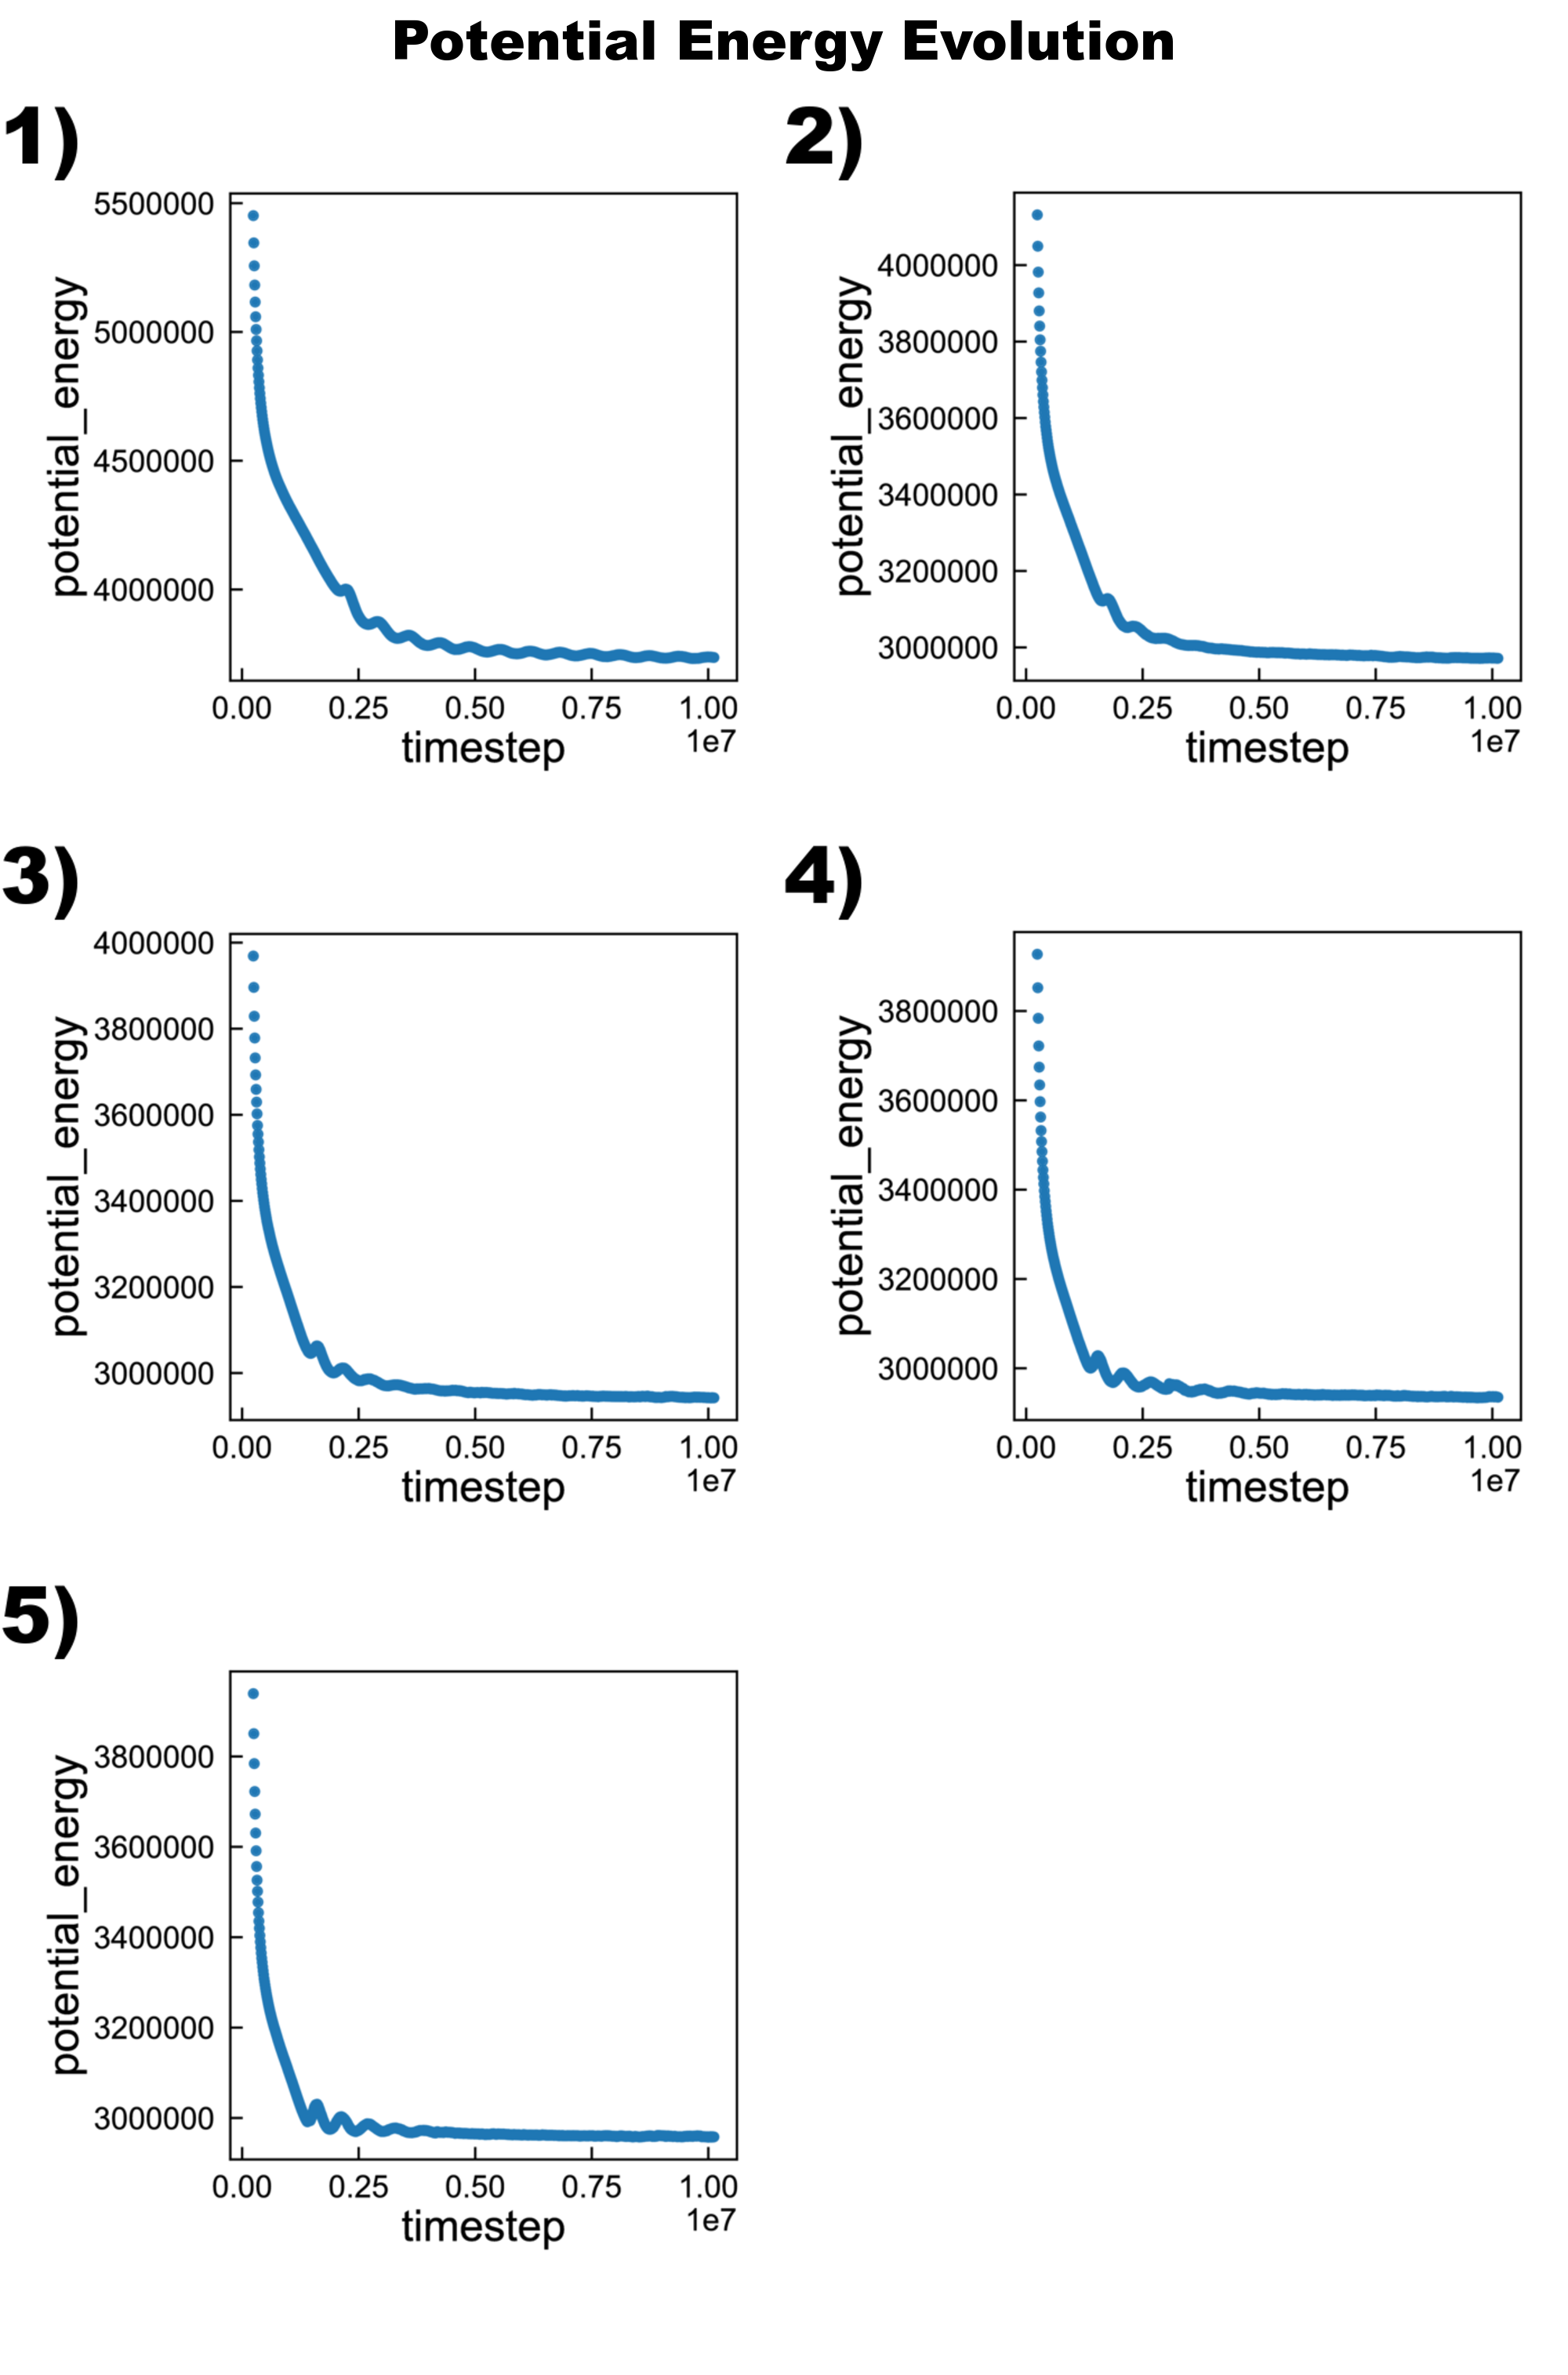
\includegraphics[width=0.7\textwidth]{Figures/Potential_Energy_Evolution.png}
    \caption{The evolution of the potential energy of the p1-L15-f0.0-P0.1-TX.X-e0.5 systems that have been run until equilibration.
        Numbers correspond to the IDs given in table \ref{table:mob}: \textbf{1}) $T = 1.5$, \textbf{2}) $T = 1.75$, \textbf{3}) $T = 2.0$, \textbf{4}) $T = 2.25$, \textbf{5}) $T = 2.5$.
    The temperature was dumped 1000 times for each phase, and only the final 990 energy values recorded are shown here.
    The final phase ran 1E7 timesteps of 1E-5s each.
}
	\label{fig:PE}
\end{figure}


\clearpage


\section{Results}


\begin{figure}[h]\centering
	\includegraphics[width=0.62\textwidth]{Figures/newFGP3HT_T1.5_Tau1.0_equil.png}
    \caption{   1) Chromophore connectivity network, 
                2) Location of `stacks', 
                3) Distribution of connected chromophore separations (defines stacks),
                4) Density of states of Frontier molecular orbital (delta Eij),
                5) KMC Carrier termination locations (defines anisotropy),
                6) Histogram of molecular transfer integrals,
                7) Histogram of stack transfer integrals,
                8) Histogram of molecular hopping rates,
                9) Histogram of stack hopping rates,
                10) Linear MSD plot,
                11) Semi-log-x MSD plot,
                12) Logarithmic MSD plot.}
	\label{fig:T1.5}
\end{figure}


\begin{figure}[h]\centering
	\includegraphics[width=0.85\textwidth]{Figures/newFGP3HT_T1.75_Tau1.0_equil.png}
    \caption{   1) Chromophore connectivity network, 
                2) Location of `stacks', 
                3) Distribution of connected chromophore separations (defines stacks),
                4) Density of states of Frontier molecular orbital (delta Eij),
                5) KMC Carrier termination locations (defines anisotropy),
                6) Histogram of molecular transfer integrals,
                7) Histogram of stack transfer integrals,
                8) Histogram of molecular hopping rates,
                9) Histogram of stack hopping rates,
                10) Linear MSD plot,
                11) Semi-log-x MSD plot,
                12) Logarithmic MSD plot.}
	\label{fig:T1.75}
\end{figure}


\begin{figure}[h]\centering
	\includegraphics[width=0.85\textwidth]{Figures/newFGP3HT_T2.0_Tau1.0_equil.png}
    \caption{   1) Chromophore connectivity network, 
                2) Location of `stacks', 
                3) Distribution of connected chromophore separations (defines stacks),
                4) Density of states of Frontier molecular orbital (delta Eij),
                5) KMC Carrier termination locations (defines anisotropy),
                6) Histogram of molecular transfer integrals,
                7) Histogram of stack transfer integrals,
                8) Histogram of molecular hopping rates,
                9) Histogram of stack hopping rates,
                10) Linear MSD plot,
                11) Semi-log-x MSD plot,
                12) Logarithmic MSD plot.}
	\label{fig:T2.0}
\end{figure}


\begin{figure}[h]\centering
	\includegraphics[width=0.85\textwidth]{Figures/newFGP3HT_T2.25_Tau1.0_equil.png}
    \caption{   1) Chromophore connectivity network, 
                2) Location of `stacks', 
                3) Distribution of connected chromophore separations (defines stacks),
                4) Density of states of Frontier molecular orbital (delta Eij),
                5) KMC Carrier termination locations (defines anisotropy),
                6) Histogram of molecular transfer integrals,
                7) Histogram of stack transfer integrals,
                8) Histogram of molecular hopping rates,
                9) Histogram of stack hopping rates,
                10) Linear MSD plot,
                11) Semi-log-x MSD plot,
                12) Logarithmic MSD plot.}
	\label{fig:T2.25}
\end{figure}


\begin{figure}[h]\centering
	\includegraphics[width=0.85\textwidth]{Figures/newFGP3HT_T2.5_Tau1.0_equil.png}
    \caption{   1) Chromophore connectivity network, 
                2) Location of `stacks', 
                3) Distribution of connected chromophore separations (defines stacks),
                4) Density of states of Frontier molecular orbital (delta Eij),
                5) KMC Carrier termination locations (defines anisotropy),
                6) Histogram of molecular transfer integrals,
                7) Histogram of stack transfer integrals,
                8) Histogram of molecular hopping rates,
                9) Histogram of stack hopping rates,
                10) Linear MSD plot,
                11) Semi-log-x MSD plot,
                12) Logarithmic MSD plot.}
	\label{fig:T2.5}
\end{figure}

%
%
%\begin{figure}[h!]\centering
%	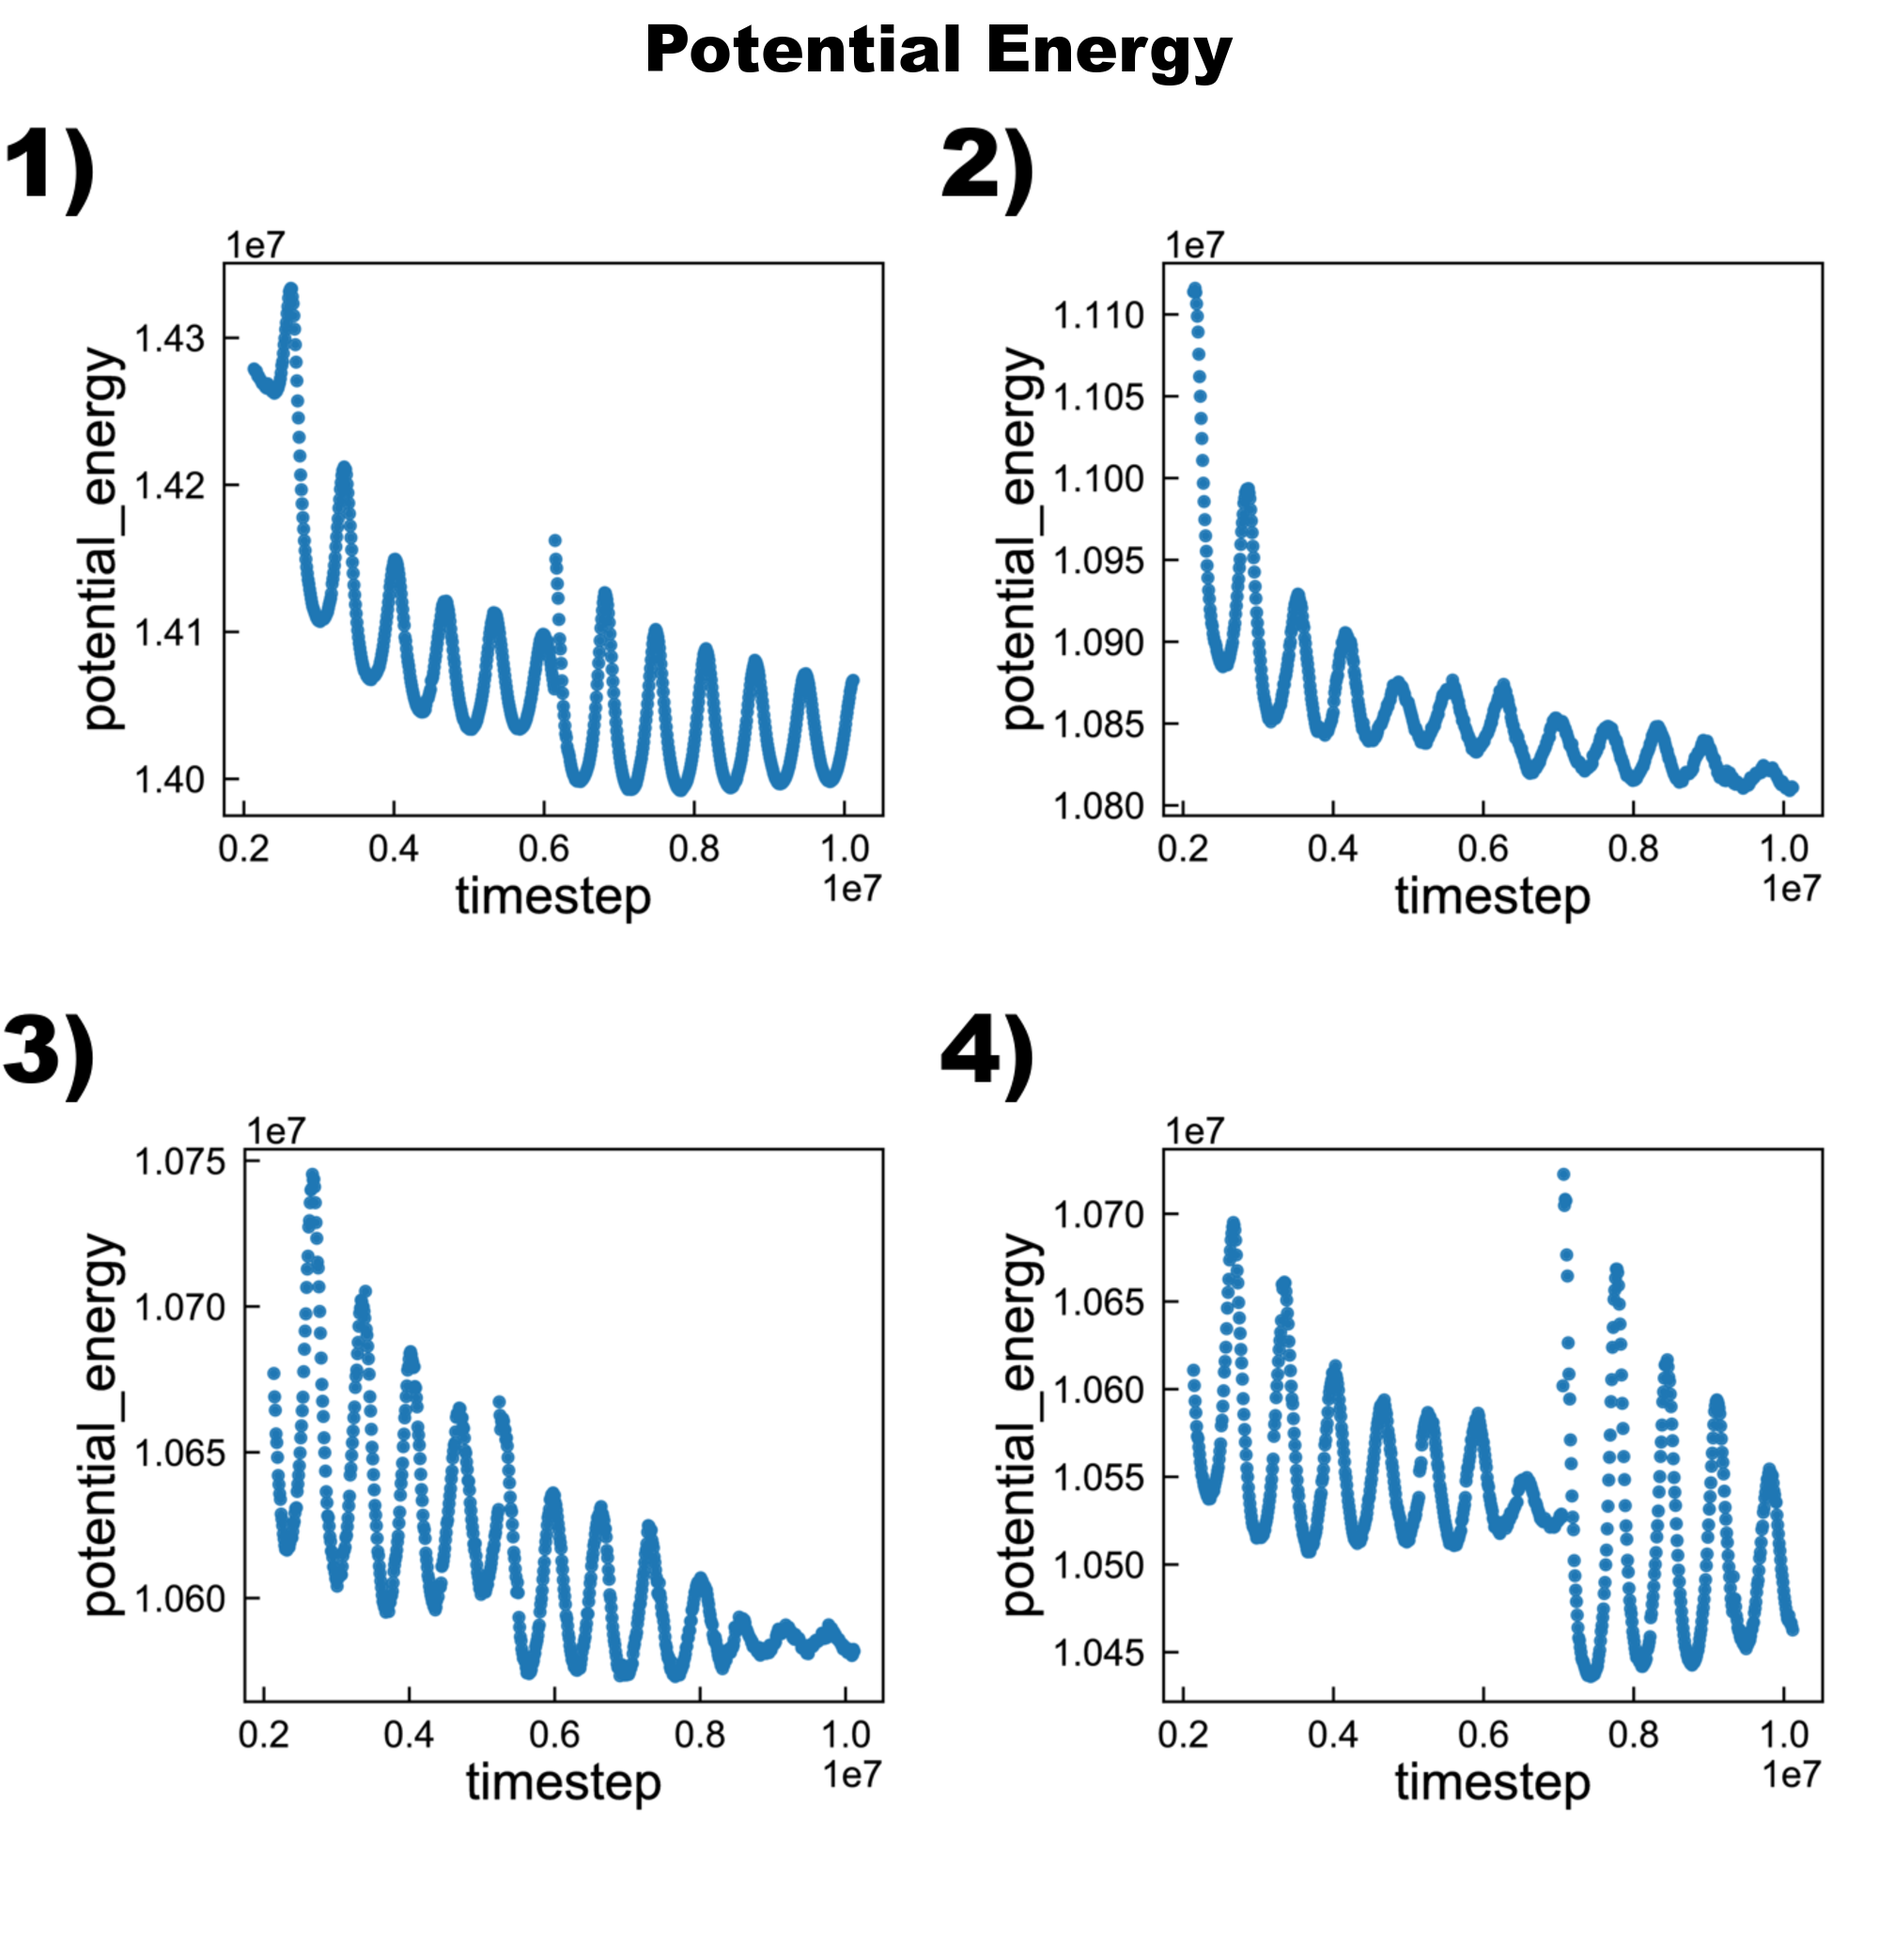
\includegraphics[width=\textwidth]{Figures/Potential_Energy.png}
%    \caption{The evolution of the total potential energy of the p1-L15-f0.0-P0.1-TX.X-e0.5 systems.
%        a) $T = 1.5$, b) $T = 1.75$, c) $T = 2.0$, d) $T = 2.25$.
%    The potential energy was dumped 1000 times for each phase, and only the final 800 energy values recorded are shown here.
%    The final phase ran 1E7 timesteps of 1E-5s each.
%}
%	\label{fig:PE}
%\end{figure}
%
%
%\textcolor{red}{Not going to report the mobilities until we are happy with the equilibration first.}


\bibliography{refs}
\bibliographystyle{unsrt}


\end{document}
